% =====================================================================
%  Noxed / SprintLab — Adaptive Learning Loop (System Flowchart)
%  Compile:  pdflatex Noxed_Flowchart.tex
% =====================================================================
\documentclass[11pt]{article}
\usepackage[a4paper,margin=1.4cm]{geometry}
\usepackage{lmodern}
\usepackage[T1]{fontenc}
\usepackage{tikz}
\usepackage{amsmath}
\usepackage{amssymb}
\usepackage{xcolor}
\usetikzlibrary{shapes.geometric,arrows.meta,positioning,calc,fit,backgrounds}

% ---- palette -------------------------------------------------------
\definecolor{cStart}{HTML}{2F4B7C}
\definecolor{cIO}{HTML}{4A7BB7}
\definecolor{cProc}{HTML}{5A6472}
\definecolor{cDiag}{HTML}{1B7F5B}   % Diagnostic module
\definecolor{cBeh}{HTML}{B5651D}    % Behavioural module
\definecolor{cBan}{HTML}{7A3B8F}    % Bandit module
\definecolor{cProg}{HTML}{2A9D8F}   % Progress module
\definecolor{cDec}{HTML}{C44536}
\definecolor{cData}{HTML}{6B7280}
\definecolor{cBG}{HTML}{F4F6F9}

% ---- node styles ---------------------------------------------------
\tikzset{
  font=\sffamily\small,
  base/.style={draw,thick,rounded corners=2pt,align=center,text=white,
               minimum height=9mm,inner sep=4pt,minimum width=32mm},
  startstop/.style={base,fill=cStart,rounded corners=10pt},
  io/.style={base,fill=cIO,trapezium,trapezium left angle=70,
             trapezium right angle=110,trapezium stretches=true},
  proc/.style={base,fill=cProc},
  mDiag/.style={base,fill=cDiag,minimum width=52mm},
  mBeh/.style={base,fill=cBeh,minimum width=52mm},
  mBan/.style={base,fill=cBan,minimum width=52mm},
  mProg/.style={base,fill=cProg,minimum width=52mm},
  decision/.style={draw,thick,fill=cDec,text=white,align=center,
                   diamond,aspect=2,inner sep=1pt,minimum width=30mm,font=\sffamily\scriptsize},
  data/.style={draw,thick,cylinder,shape border rotate=90,aspect=0.25,
               fill=cData,text=white,align=center,minimum height=11mm,minimum width=26mm,font=\sffamily\scriptsize},
  flow/.style={-{Stealth[length=3mm]},thick,cProc},
  fb/.style={-{Stealth[length=3mm]},thick,dashed,cDec},
  lbl/.style={font=\sffamily\scriptsize\itshape,text=cProc},
  modtag/.style={font=\sffamily\bfseries\scriptsize,text=black,fill=cBG,inner sep=2pt},
}

\begin{document}
\pagestyle{empty}
\begin{center}
{\sffamily\bfseries\large Noxed --- Adaptive Learning Loop for Egyptian School Science}\\[1pt]
{\sffamily\footnotesize Diagnose knowledge \& behaviour $\rightarrow$ recommend the next question/level $\rightarrow$ track progress $\rightarrow$ repeat}
\end{center}
\vspace{2mm}

\begin{center}
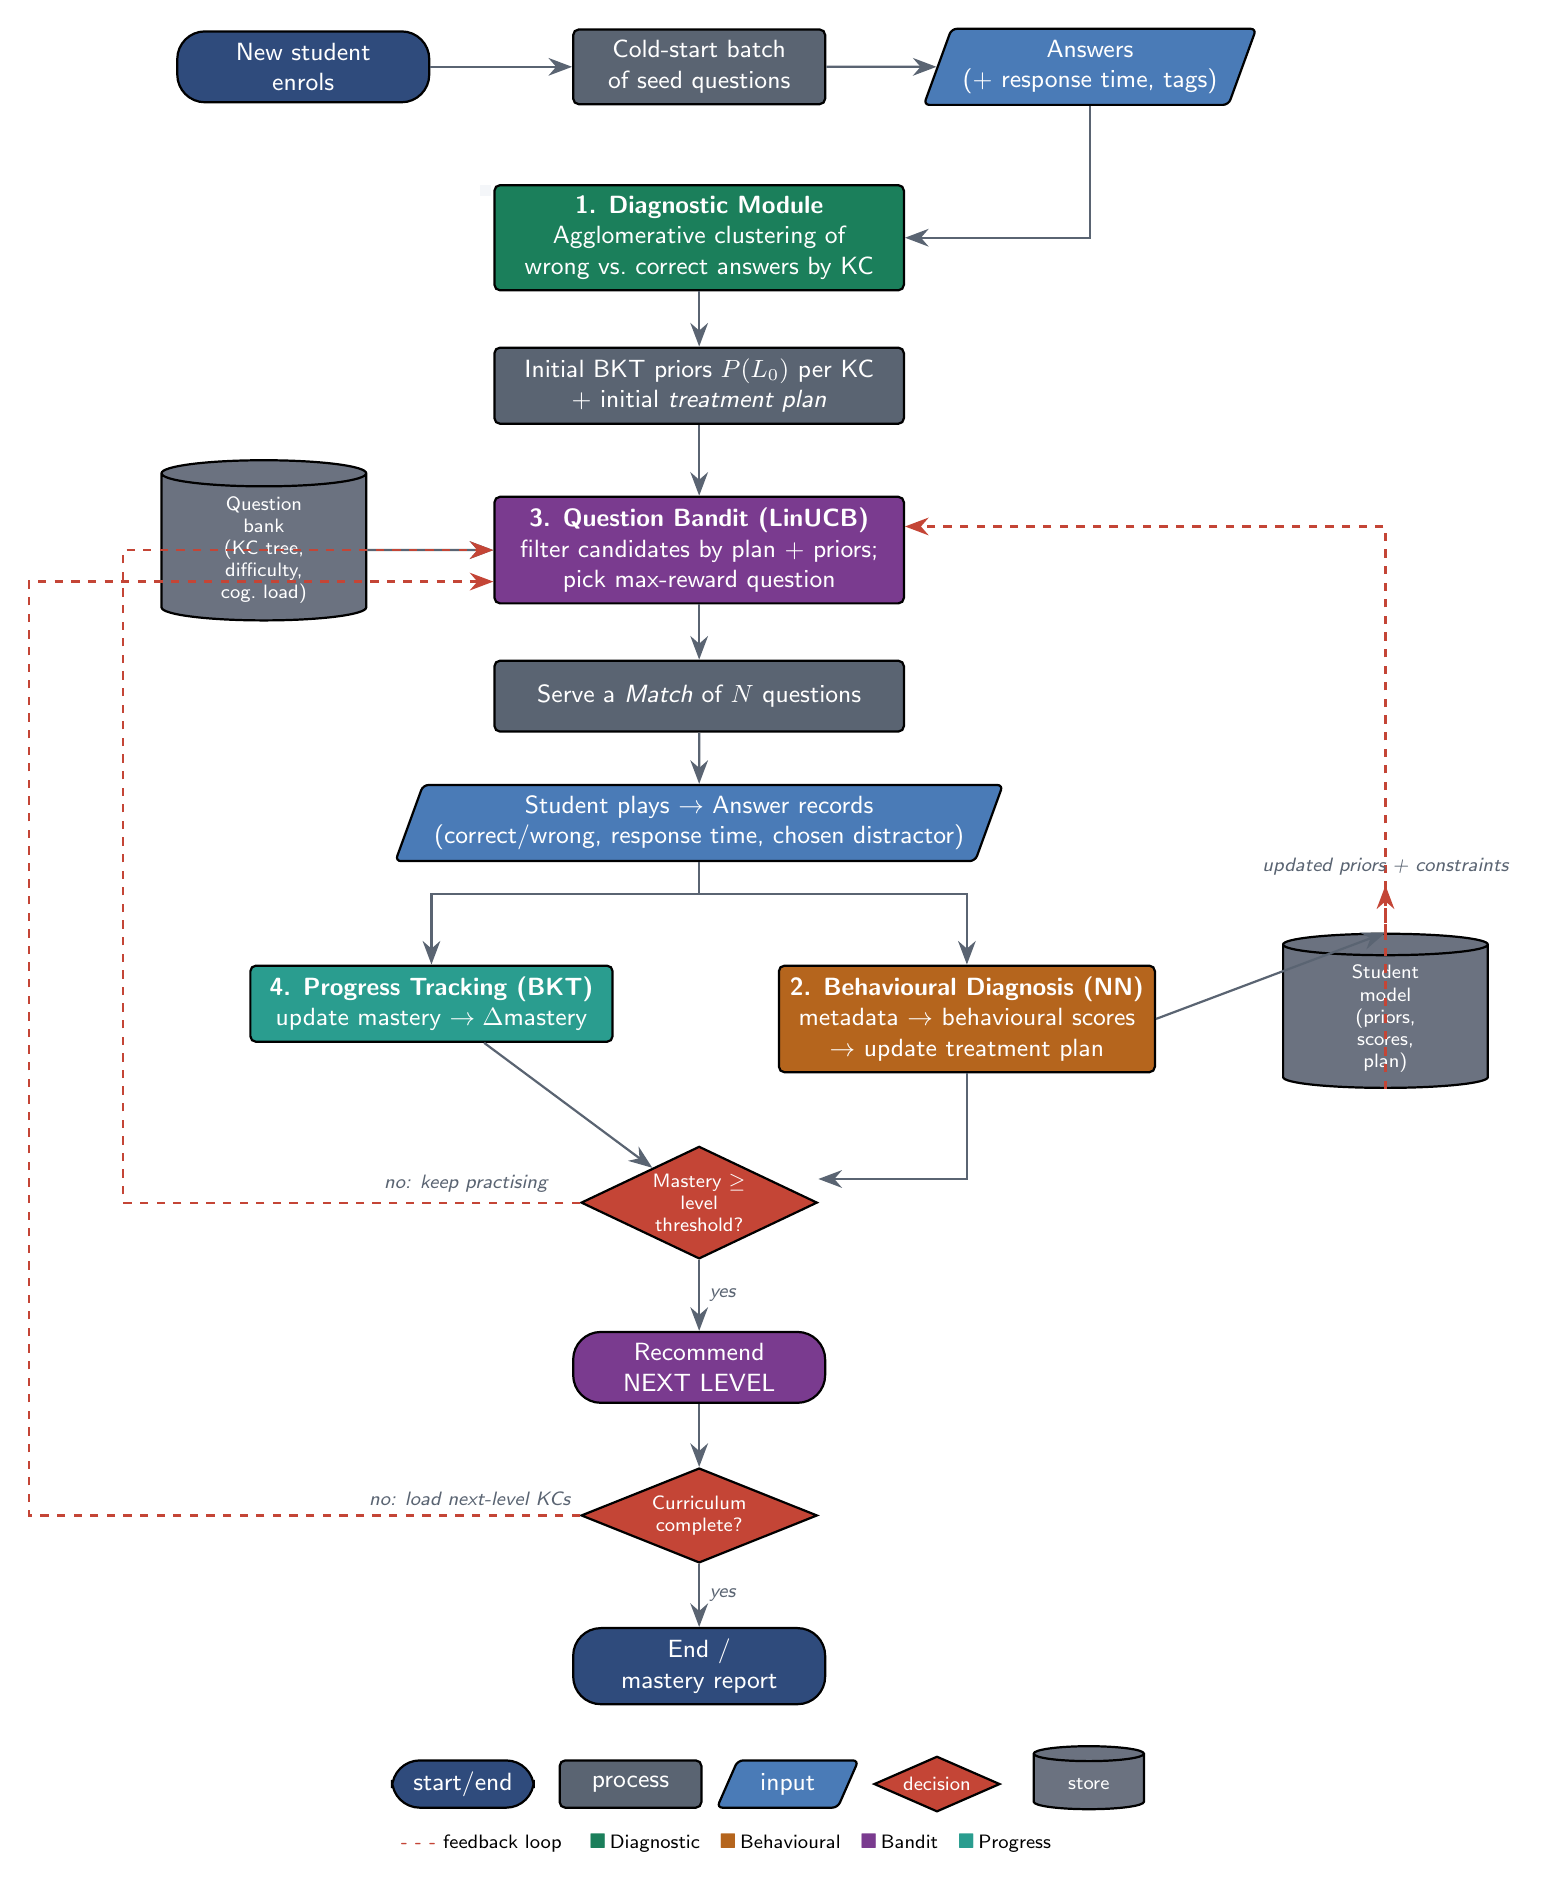
\begin{tikzpicture}[node distance=6.5mm and 14mm]

% ============ COLD START (top) ============
\node[startstop] (start) {New student\\ enrols};
\node[proc, right=18mm of start] (cold) {Cold-start batch\\ of seed questions};
\node[io, right=14mm of cold] (ans0) {Answers\\ (+ response time, tags)};

% ============ DIAGNOSTIC MODULE ============
\node[mDiag, below=10mm of cold] (diag)
   {\textbf{1. Diagnostic Module}\\ Agglomerative clustering of\\ wrong vs.\ correct answers by KC};
\node[proc, below=7mm of diag, minimum width=52mm] (priors)
   {Initial BKT priors $P(L_0)$ per KC\\ + initial \emph{treatment plan}};

% ============ QUESTION BANDIT ============
\node[mBan, below=9mm of priors] (bandit)
   {\textbf{3. Question Bandit (LinUCB)}\\ filter candidates by plan + priors;\\ pick max-reward question};
\node[data, left=16mm of bandit] (qbank) {Question\\ bank\\ (KC tree,\\ difficulty,\\ cog.\ load)};

% ============ SERVE + PLAY ============
\node[proc, below=7mm of bandit, minimum width=52mm] (serve) {Serve a \emph{Match} of $N$ questions};
\node[io, below=6.5mm of serve, minimum width=52mm] (play)
   {Student plays $\rightarrow$ Answer records\\ (correct/wrong, response time, chosen distractor)};

% ============ PROGRESS + BEHAVIOURAL (parallel) ============
\node[mProg, below=13mm of play, xshift=-34mm, minimum width=46mm] (prog)
   {\textbf{4. Progress Tracking (BKT)}\\ update mastery $\rightarrow \Delta$mastery};
\node[mBeh, below=13mm of play, xshift=34mm, minimum width=46mm] (beh)
   {\textbf{2. Behavioural Diagnosis (NN)}\\ metadata $\rightarrow$ behavioural scores\\ $\rightarrow$ update treatment plan};

% ============ DECISIONS ============
\node[decision, below=13mm of prog, xshift=34mm] (dmastery) {Mastery $\ge$\\ level\\ threshold?};
\node[startstop, fill=cBan, below=9mm of dmastery] (level) {Recommend\\ NEXT LEVEL};
\node[decision, below=8mm of level] (ddone) {Curriculum\\ complete?};
\node[startstop, below=8mm of ddone] (end) {End /\\ mastery report};

% student model store
\node[data, right=16mm of beh] (smodel) {Student\\ model\\ (priors,\\ scores,\\ plan)};

% ---------- edges: cold start ----------
\draw[flow] (start) -- (cold);
\draw[flow] (cold) -- (ans0);
\draw[flow] (ans0.south) |- (diag.east);
\draw[flow] (diag) -- (priors);
\draw[flow] (priors) -- (bandit);
\draw[flow] (qbank) -- (bandit);
\draw[flow] (bandit) -- (serve);
\draw[flow] (serve) -- (play);

% ---------- edges: to parallel modules ----------
\draw[flow] (play.south) -- ++(0,-4mm) -| (prog.north);
\draw[flow] (play.south) -- ++(0,-4mm) -| (beh.north);

% ---------- edges: modules to decision / store ----------
\draw[flow] (prog) -- (dmastery);
\draw[flow] (beh.east) -- (smodel.north);
\draw[flow] (beh.south) |- ($(dmastery.east)+(0,3mm)$);

% ---------- decision outcomes ----------
\draw[flow] (dmastery) -- node[lbl,right]{yes} (level);
\draw[flow] (level) -- (ddone);
\draw[flow] (ddone) -- node[lbl,right]{yes} (end);

% ---------- FEEDBACK LOOPS (dashed) ----------
% mastery not reached -> keep practising this level (back to bandit)
\draw[fb] (dmastery.west) -- node[lbl,above,pos=0.25]{no: keep practising}++(-58mm,0) |- (bandit.west);
% next level not done -> back to bandit with new KCs
\draw[fb] (ddone.west) -- node[lbl,above,pos=0.2]{no: load next-level KCs}++(-70mm,0) |- ($(bandit.west)-(0,4mm)$);
% updated student model feeds the bandit's next decision
\draw[fb] (smodel.south) |- ($(bandit.east)+(0,3mm)$);
\draw[fb] (smodel.north) -- ++(0,6mm) node[lbl,above]{updated priors + constraints};

% ---------- module band tags ----------
\node[modtag,left=1mm of diag.north west, anchor=east, rotate=90] {};

% ---------- legend ----------
\begin{scope}[shift={($(end.south)+(-30mm,-10mm)$)}]
  \node[startstop,minimum width=18mm,minimum height=6mm] (l1) {start/end};
  \node[proc,right=3mm of l1,minimum width=18mm,minimum height=6mm] (l2) {process};
  \node[io,right=3mm of l2,minimum width=18mm,minimum height=6mm] (l3) {input};
  \node[decision,right=3mm of l3,minimum width=16mm] (l4) {decision};
  \node[data,right=4mm of l4,minimum width=14mm,minimum height=8mm] (l5) {store};
  \node[below=2mm of l1.south west,anchor=north west,font=\sffamily\scriptsize] {%
    \textcolor{cDec}{\textbf{- - -}} feedback loop \quad
    \textcolor{cDiag}{$\blacksquare$}\,Diagnostic \;
    \textcolor{cBeh}{$\blacksquare$}\,Behavioural \;
    \textcolor{cBan}{$\blacksquare$}\,Bandit \;
    \textcolor{cProg}{$\blacksquare$}\,Progress};
\end{scope}

\end{tikzpicture}
\end{center}

\end{document}
